\documentclass{book}
\usepackage{commeunjeustyle}
\usepackage{pgf,tikz,tkz-euclide}
\usetikzlibrary{decorations.pathmorphing} 
\usepackage{tkz-euclide}
\usetikzlibrary{calc,intersections,through,backgrounds,snakes}
\usepackage{pgfplots}
\usepackage{tkz-euclide}
\usetikzlibrary{calc,intersections}
\begin{document}
\chapter*{Intégrales généralisées}
Ce chapitre a pour objectif d'étendre la notion d'intégrale sur un intervalle qui n'est pas nécessairement un
segment, par exemple, $$\int_{1 }^{+\infty } \frac{1}{x^2} \,\mathrm dx = 1.$$
\begin{center}
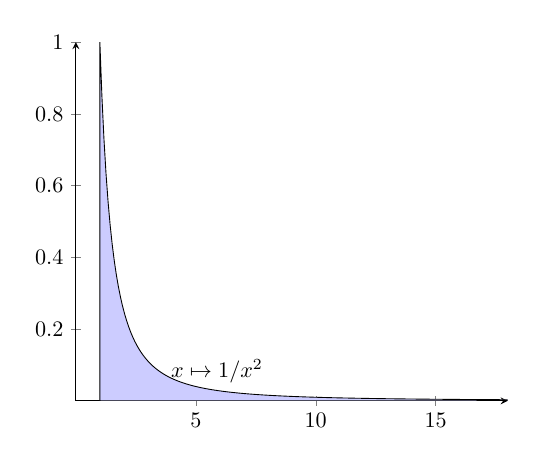
\begin{tikzpicture}[scale=0.8]
\begin{axis}[
	   axis y line = middle,
       axis x line = middle,
       samples     = 200,
       domain      = 0:1,
       xmin = 0, xmax = 18,
       ymin = 0, ymax = 1,
]
\addplot[domain=1:18,fill=blue!20] {1/x^2} node[pos=0.3,above] {$x\mapsto 1/x^2$}\closedcycle ;
\end{axis}
\end{tikzpicture}
\end{center}
\section{Généralités}
L'intégrale impropre désigne l'intégrale d'une fonction sur un intervalle. Elle est définie comme une extension de l'intégrale usuelle sur un segment  par un passage à la limite sur les bornes d'intégration de l'intégrale.   

\subsection{Définition}
\begin{Definition}[Intégrale impropre sur $[a,b[$]
Soit $f$ une fonction continue par morceaux sur $[a,b [$ avec $b \in \R$ ou $b = +\infty$.\\
Si $\int_a^t f(x) \,\mathrm dx$ admet une limite finie lorsque $t$ tend vers $b$, on dit que l'\defi{intégrale impropre} converge et on
note $\int_a^b f(x) \,\mathrm dx$ cette limite. Sinon, on dit qu'elle diverge.
\end{Definition}
\begin{Exemple}
Soit l'intégrale $\int_1^{+\infty } \frac{1}{x^2}\,\mathrm dx$.\\
La fonction $ x\mapsto  \frac{1}{x^2}$ est continue sur $[1,{+\infty }[$.\\ 
Soit $t\in [1,{+\infty }[$.\\
On a  $\int_1^t \frac{1}{x^2}\,\mathrm dx=[-\frac 1 x]_1^t=1-\frac{1}{t}\xrightarrow[t\to+\infty ]{}1$.\\
L'intégrale est convergente et son intégrale impropre est égale à 1.
\end{Exemple}
\begin{Proposition}[Indépendance de la borne fermée]
Soit $f$ une fonction continue par morceaux sur $[a,b [$ avec $b \in \R$ ou $b = +\infty$. Soit $c\in[a,b[$.\\
$\int_a^b f(x) \,\mathrm dx$ et $\int_c^b f(x) \,\mathrm dx$ sont de même nature.
\end{Proposition}
\begin{Demonstration}
Soit $t\in[a,b[$. On applique la relation de Chasles à l'intégrale sur un segment :
$$ \int_a^t f(x) \,\mathrm dx = \int_a^c f(x) \,\mathrm dx+\int_c^t f(x) \,\mathrm dx=A+\int_c^t f(x) \,\mathrm dx.$$
Par passage à la limite sur cette égalité, on obtient que $\int_a^b f(x) \,\mathrm dx$ et $\int_c^b f(x) \,\mathrm dx$ sont de même nature.
\end{Demonstration}
\begin{Exemple}
$\int_5^{+\infty } \frac{1}{x^2}\,\mathrm dx$ converge car $\int_1^{+\infty } \frac{1}{x^2}\,\mathrm dx$ converge.
\end{Exemple}

\begin{Definition}[Intégrale impropre sur {$]a,b]$}]
Soit $f$ une fonction continue par morceaux  sur $]a,b]$ avec $a \in \R$ ou $a= -\infty$.\\
Si $\int_t^b f(x) \,\mathrm dx$ admet une limite finie lorsque $t$ tend vers $a$, on dit que l'\defi{intégrale impropre} converge et on
note $\int_a^b f(x) \,\mathrm dx$ cette limite. Sinon, on dit qu'elle diverge.
\end{Definition}
\begin{Exemple}
Soit l'intégrale $\int_0^{1} \frac{1}{x}\,\mathrm dx$.\\
La fonction $ x\mapsto  \frac{1}{x}$ est continue sur $]0,1]$.  Soit $t\in ]0,1]$.\\
On a  $\int_t^1 \frac{1}{x}\,\mathrm dx=[\ln (x)]_t^1=-\ln(t)\xrightarrow[t\to 0 ]{}+\infty$. Donc l'intégrale est divergente.
\end{Exemple}
\begin{Definition}[Intégrale impropre sur {$]a,b[$}]
Soit $f$ une fonction continue par morceaux  sur $]a,b[$ avec $a \in \R$ ou $a= -\infty$ et $b \in \R$ ou $b= +\infty$ .\\
Si $\int_a^c f(x) \,\mathrm dx$ et $\int_c^b f(x) \,\mathrm dx$  convergent avec $c\in ]a,b[$, on dit que l'\defi{intégrale impropre} converge et on
note $\int_a^b f(x) \,\mathrm dx$ cette limite. Sinon, on dit qu'elle diverge.
\end{Definition}
\begin{Exemple}
Soit l'intégrale $\int_0^{+\infty } \frac{1}{\sqrt{x}}\,\mathrm dx$.\\
La fonction $ x\mapsto  \frac{1}{x^2}$ est continue sur $]0,+\infty[$. \\
\begin{itemize}
\item \textit{En 0 :}   Soit $t\in ]0,1]$.\\
On a  $\int_t^1 \frac{1}{\sqrt{x}}\,\mathrm dx=[2 \sqrt{x}]_t^1=2(1-\sqrt{t})\xrightarrow[t\to 0 ]{}2$.\\Donc l'intégrale $\int_0^1  \frac{1}{\sqrt{x}}\,\mathrm dx$  est convergente.
\item \textit{En $+\infty$ :} Soit $t\in [1,{+\infty }[$.\\
On a  $\int_1^t \frac{1}{\sqrt{x}}\,\mathrm dx=[2 \sqrt{x}]_1^t=2(\sqrt{t}-1)\xrightarrow[t\to +\infty ]+\infty $.\\Donc l'intégrale $\int_1^{+\infty } \frac{1}{\sqrt{x}}\,\mathrm dx$ est divergente.
\end{itemize}
En conclusion,  l'intégrale $\int_0^{+\infty } \frac{1}{\sqrt{x}}\,\mathrm dx$ est divergente.
\end{Exemple}
\begin{Remarque}
Attention au passage à la limite! Pour prouver que $\int_{-\infty}^{+\infty}f(x)\,\mathrm dx$ converge, il ne suffit pas de calculer $\lim\limits_{t\to +\infty }\int_{-t}^t f(x)\,\mathrm dx$.\\
En effet soit $\int_{-\infty}^{+\infty} {x}\,\mathrm dx.$\\
On a:
\begin{enumerate}
\item
  $x\mapsto x$ est continue sur $]-\infty ,+\infty [$,
\item
  $\lim\limits_{t\to +\infty }\int_{-t}^t x\,\mathrm dx =\lim\limits_{t\to +\infty } [\frac{x^2}{2}]_t^t=0  $ existe et est nulle,
\item
  pourtant, l'intégrale $\int_{-\infty }^{+\infty } x\,\mathrm dx$ diverge car $\int_{0 }^{+\infty } x\,\mathrm dx$ est divergente.
\end{enumerate}
\begin{center}
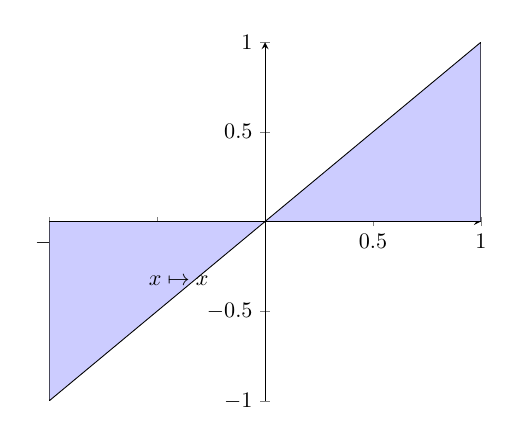
\begin{tikzpicture}[scale=0.8]
\begin{axis}[
	   axis y line = middle,
       axis x line = middle,
       samples     = 200,
       domain      = -1:1,
       xmin = -1, xmax = 1,
       ymin = -1, ymax = 1,
]
\addplot[domain=-1:1,fill=blue!20] {x} node[pos=0.3,above] {$x\mapsto x$}\closedcycle ;
\end{axis}
\end{tikzpicture}
\end{center}
\end{Remarque}

\begin{Proposition}[Prolongeable par continuité]
Si une fonction $f : [a,b [\to \R$ avec $b \in \R$ est continue sur $[a,b [$ et prolongeable par continuité en $b$,\\
Alors l'intégrale $\int_{a}^{b}f(x)\,\mathrm dx$ converge et vaut $\int_{a}^{b}\tilde{f}(x)\,\mathrm dx$ où l'on a noté $\tilde{f}$ le prolongement de $f$. L'intégrale est faussement impropre.
\end{Proposition}
\begin{Demonstration}
Soit $f$ une  fonction continue sur $[a,b[$ prolongeable par continuité en $b$. On note $\tilde{f}$ le prolongement de $f$.\\
Comme $\tilde{f}$ est continue sur $[a,b]$, $\tilde{f}$ admet une primitive $\Phi$ sur $[a, b]$. Soit $t \in [a, b[$.
$$\begin{aligned}
\int_{a}^{t}f(x)\,\mathrm dx&=\int_{a}^{t}\tilde{f}(x)\,\mathrm dx& \text{ car }\forall x \in [a,b[:f(x)=\tilde{f}(x)\\
\int_{a}^{t}f(x)\,\mathrm dx&=\Phi(t)- \Phi(a)\xrightarrow[t\to b ]{}\Phi(b)- \Phi(a)=\int_{a}^{b}\tilde{f}(x)\,\mathrm dx &\text{ car }\Phi  \text{ est continue sur }[a,b]\\
\end{aligned}$$
L'intégrale  $\int_{a}^{b}f(x)\,\mathrm dx$ converge de limite  $\int_{a}^{b}\tilde{f}(x)\,\mathrm dx$.
\end{Demonstration}
\begin{Exemple}
L'intégrale $\int_{0}^{2\pi}\frac{\sin x}{x}\,\mathrm dx$ est convergente car la fonction $f:x\mapsto\frac{\sin x}{x}$ est continue sur $]0,2\pi]$ et plongeable par continuité en 0 en posant $\tilde{f}(0)=1$. 
\begin{center}
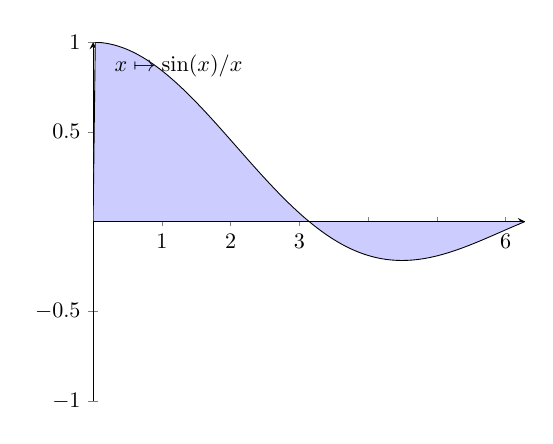
\begin{tikzpicture}[scale=0.8]
\begin{axis}[
	   axis y line = middle,
       axis x line = middle,
       samples     = 200,
       domain      = 0:1,
       xmin = 0, xmax = 6.28,
       ymin = -1, ymax = 1,
]
\addplot[domain=0:6.28,fill=blue!20] {sin(deg(x))/x} node[pos=0.3,above] {$x\mapsto \sin(x)/x$}\closedcycle ;
\end{axis}
\end{tikzpicture}
\end{center}
\end{Exemple}
Par analogie sur les séries numériques, si  $\lim\limits_{n\to \infty}u_n \neq 0$ alors $\sum u_n$ diverge, a-t-on
si $\lim\limits_{x\to \infty}f(x)\neq 0$  alors  $\int_{0}^{+\infty}f(x)\,\mathrm dx$ diverge ?\\
 La réponse est oui à condition d'avoir une hypothèse plus forte. 
\begin{Theoreme}[Divergence grossière à l'infini]
Soit $f : [a,+\infty[ \to \R$ continue.\\
Si $f$ admet une limite non nulle en $\infty$ alors $\int_{0}^{+\infty}f(x)\,\mathrm dx$ diverge. On dit qu'elle \defi{diverge grossièrement}. 
\end{Theoreme}
\begin{Demonstration}
La preuve anticipe les outils mis en place dans la section sur les fonctions positives.\\ 
Comme $f$ admet une limite $l$ non nulle en $\infty$, il existe $A>0$ tel que $f(x)$ soit de signe constant pour tout $x>A$.  Comme $f(x)\underset{+\infty}{\sim} l$ et $\int_{A}^{+\infty}l\,\mathrm dx$ diverge,  $\int_{0}^{+\infty}f(x)\,\mathrm dx$ diverge.  
\end{Demonstration} 
\begin{Exemple}
$\int_{0}^{+\infty}x\sin(1/x)\,\mathrm dx$ diverge grossièrement car $\lim\limits_{x\to+\infty}x\sin(1/x) =1 $.
\end{Exemple}

\subsection{Intégrales de références}

\begin{Proposition}[Intégrales de Riemann]
  \begin{enumerate}
  \item
    $\int_1^{+\infty } \frac{\,\mathrm dx}{x^\alpha}$ converge si et seulement si $\alpha>1$,
  \item
    $\int_0^1    \frac{\mathrm dx}{x^\alpha}$ converge si et seulement si $\alpha<1$.
  \end{enumerate}
\end{Proposition}
\begin{Demonstration}
$x\mapsto  \frac{1}{x^\alpha}$ est continue sur  $[1,+\infty[$.\\
Soit $t\in [1,+\infty[$. On a 
\begin{itemize}
\item $\alpha\neq 1$
$$\int_1^{t } \frac{\mathrm dx}{x^\alpha}= \left[\frac{x^{1-\alpha}}{1-\alpha}\right]_1^t=\frac{1}{1-\alpha}(t^{1-\alpha}-1) \xrightarrow[t\to +\infty ]{}\begin{cases}\frac{1}{\alpha-1} &\text{ si } \alpha>1\\ +\infty &\text{ si } \alpha<1 \end{cases}$$
\item $\alpha= 1$
$$\int_1^{t } \frac{\mathrm dx}{x}= \left[\ln(x)\right]_1^t=\ln(t)\xrightarrow[t\to +\infty ]{}+\infty $$
\end{itemize}
En conclusion $\int_1^{+\infty } \frac{\mathrm dx}{x^\alpha}$ converge si et seulement si $\alpha>1$.\\
La démonstration est similaire pour $\int_0^1    \frac{\mathrm dx}{x^\alpha}$ converge si et seulement si $\alpha<1$.
\end{Demonstration}
\begin{Proposition}[Exponentielle et logarithme]
  \begin{itemize}
  \item
    $\int_0^{+\infty } e^{-\alpha x} \,\mathrm dx$ converge si et seulement si $\alpha>0$,
  \item
    $\int_0^1   \ln(x) \,\mathrm dx $ converge.
  \end{itemize}
\end{Proposition}
\begin{Demonstration}
La fonction $ x\mapsto \ln(x) $ est continue sur $]0,1]$. Soit $t\in ]0,1]$.\\
$$\int_t^1   \ln(x) \,\mathrm dx \overbrace{=}^{\text{IPP avec }u(x)=\ln(x), v'(x)=1}[\ln(x)x]_t^1- \int_t^1   \frac 1 x x \,\mathrm dx= -\ln(t)t+(t-1)\xrightarrow[t\to 0 ]{} -1\text{ par croissance comparée}.$$
Donc $\int_0^1   \ln(x) \,\mathrm dx$ est convergente. 
\end{Demonstration}
\subsection{Propriétés}
\begin{Proposition}[Linéarité]
Soit $f$ et $g$ deux fonctions continues par morceaux de $[a,b[$ dans $\K$ et $\lambda,\mu\in\R$.\\
 Si les intégrales $\int_a^b f(x)\,\mathrm dx$ et $\int_a^b g(x)\,\mathrm dx$ convergent, alors l'intégrale $\int_a^b (\lambda f(x) +\mu g(x))\,\mathrm dx$ converge et on a
 $$\int_a^b (\lambda f(x) +\mu g(x))\,\mathrm dx=\lambda \int_a^b f(x)\,\mathrm dx +\mu \int_a^b g(x)\,\mathrm dx.$$
\end{Proposition}
\begin{Demonstration}
Les fonctions $f$ et $g$ sont continues sur $[a,b[$. Soit $t\in [a,b[$.\\
On a $$\int_a^t (\lambda f(x) +\mu g(x))\,\mathrm dx\overbrace{=}^{\text{linéarité sur un segment}}\lambda \int_a^t f(x)\,\mathrm dx +\mu \int_a^t g(x)\,\mathrm dx\xrightarrow[t\to b^-]{}\lambda \int_a^b f(x)\,\mathrm dx +\mu \int_a^b g(x)\,\mathrm dx.$$
Donc l'intégrale $\int_a^b (\lambda f(x) +\mu g(x))\,\mathrm dx$ converge et l'égalité.
\end{Demonstration}
\begin{Exemple}
On peut écrire
$$ \int _{1}^{+\infty }\left({\frac {1}{x^{2}}}-{\rm {e}}^{-x}\right)\,\,\mathrm {d} x=\int _{1}^{+\infty }{\frac {1}{x^{2}}}\,\mathrm {d} x-\int _{1}^{+\infty }{\rm {e}}^{-x}\,\mathrm {d} x$$
car les intégrales $\int _{1}^{+\infty }{\frac {1}{x^{2}}}\,\mathrm {d} x $ et  $\int _{1}^{+\infty }{\rm {e}}^{-x}\,\mathrm {d} x$  convergent.\\
En revanche on ne peut pas écrire
$$ \int _{1}^{+\infty }{\frac {1}{x(x+1)}}\,\mathrm {d} x=\int _{1}^{+\infty }\frac {1}{x}\,\mathrm {d} x-\int _{1}^{+\infty }\frac {1}{x+1}\,\mathrm {d} x.$$
car l'intégrale $\int _{1}^{+\infty }\frac {1}{x}\,\mathrm {d} x$ diverge. \\
Ici il faut intégrer sur le segment $[a, t ]$ avec $t\in [a,b [$ avant de passer à la limite. On a :
$$ \int _{1}^{t }{\frac {1}{x(x+1)}}\,\mathrm {d} x=\int _{1}^{t }\frac {1}{x}\,\mathrm {d} x-\int _{1}^{t }\frac {1}{x+1}\,\mathrm {d} x=\ln(2)+\ln\left(\frac{t}{1+t}\right)=\ln(2)-\ln\left(1+\frac 1 t\right)\xrightarrow[t\to +\infty]{}\ln(2).$$
\end{Exemple}
\begin{Corollaire}[Cas complexe]
Soit $f$  continue par morceaux de $[a,b[$ dans $\C$.\\
$\int_a^b Re(f(x))\mathrm dx$  et $\int_a^b Im(f(x))\,\mathrm dx$ convergent si et seulement si $\int_a^b f(x)\,\mathrm dx$.\\
Dans ce cas 
$$ \int_a^b f(x)\,\mathrm dx = \int_a^b Re(f(x))\,\mathrm dx+ i \int_a^b Im(f(x))\,\mathrm dx.$$
\end{Corollaire}
\begin{Proposition}[Relation de Chasles]
Soit $f$ une fonction continue par morceaux de $]a,b[$ dans $\K$ telle que $\int_a^b f(x)\,\mathrm dx$ converge.\\
Alors, pour tout $c\in ]a,b[$, on a $$ \int_a^b f(x)\,\mathrm dx =\int_a^c f(x)\,\mathrm dx+\int_c^b f(x)\,\mathrm dx.$$
\end{Proposition}
\begin{Proposition}[Positivité]
Soit $f$ une fonction continue de $[a,b[$ dans $\K$ et positive telle que $\int_a^b f(x)\,\mathrm dx$ converge.\\
Alors, $ \int_a^b f(x)\,\mathrm dx \geq 0.$\\
De plus, si  $ \int_a^b f(x)\,\mathrm dx =0$ alors $f=0$, c'est à dire $f(x)=0,\forall x \in [a,b[$.
\end{Proposition}
\begin{Demonstration}
De nouveau, il faut intégrer sur le segment $[a, t]$ avec $t\in [a,b [$  
$$\int_a^t  f(x)\,\mathrm dx\overbrace{\geq}^{\text{positivité sur un segment}} 0$$
puis le passage à la limite.
\end{Demonstration}
\begin{Corollaire}[Croissance]
Soit $f$ et $g$ deux fonctions continues par morceaux de $[a,b[$ telles que les intégrales $\int_a^b f(x)\,\mathrm dx$ et $\int_a^b g(x)\,\mathrm dx$ convergent.\\
Si $\forall x\in [a,b[:\quad  f(x)\leq  g(x)$,
Alors $\int_a^b f(x)\,\mathrm dx \leq  \int_a^b g(x)\,\mathrm dx$.
\end{Corollaire}
\begin{Demonstration}
Comme $g-f\geq 0$, du fait de la positivité et de la linéarité de l'intégrale, on  a  $\int_a^b f(x)\,\mathrm dx \leq  \int_a^b g(x)\,\mathrm dx$.
\end{Demonstration}
\subsection{Calcul d'intégrale}
\begin{Theoreme}[Changement de variables]
Soit $f:]a,b]\to \K $ une fonction continue par morceaux, $\phi:[\alpha,\beta[\to  [a,b[$ une bijection strictement croissante de classe $C^1$.\\
Alors l'intégrale
$\int_\alpha^\beta f(\phi(x))\phi'(x)\,\mathrm dx $ est convergente si et seulement si $\int_a^b f(x)\,\mathrm dx$ est convergente. En cas de convergence, on a l'égalité :
$$\int_\alpha^\beta f(\phi(x))\phi'(x)\,\mathrm dx =\int_a^b f(x)\,\mathrm dx$$
\end{Theoreme}
\begin{Demonstration}
Supposons que $\int_a^b f(x)\,\mathrm dx$ converge.\\
Soit $t\in[\alpha,\beta[.$ Par changement de variable sur le
segment $[\alpha , t]$, 
$$\int_\alpha^t f(\phi(x))\phi'(x)\,\mathrm dx =\int_a^{\phi(t)} f(x)\,\mathrm dx.$$
Comme $\phi$ est une bijection croissante, $\phi(t )\xrightarrow[t \to \beta]{} b$. Donc par passage à la limite, 
$$\int_\alpha^t f(\phi(x))\phi'(x)\,\mathrm dx\xrightarrow[t \to \beta ]{} \int_a^b f(x)\,\mathrm dx.$$
Donc $\int_\alpha^\beta f(\phi(x))\phi'(x)\,\mathrm dx $ converge et est égale à  $\int_a^b f(x)\,\mathrm dx$.
Idem si l'on suppose que $\int_\alpha^\beta f(\phi(x))\phi'(x)\,\mathrm dx$ converge.
\end{Demonstration}
\begin{Exemple}
Calculons l'intégrale $\int_0^{+\infty}\frac{\ln x}{1+x^2}\,\mathrm dx$.\\
On suppose que l'intégrale converge (voir la prochaine sous-section pour la démonstration).\\
Le changement de variables $u=1/t$ donne :
$$\int^{+\infty }_0 \frac{\ln x}{1+x^2}\,\mathrm dx=\int^{0}_{+\infty } \frac{-\ln u}{1+1/u^2}\frac{-1}{u^2}\,\mathrm du=-\int^{+\infty }_0 \frac{\ln u}{1+u^2}\,\mathrm du.$$
On en déduit que $\int_0^{+\infty}\frac{\ln x}{1+x^2}\,\mathrm dx=0$.
\end{Exemple}
\begin{Theoreme}[Intégration par parties]
Soit $u$ et $v$ deux fonctions $[a,b[ \to\K $ dérivables telles que $u'$ et $v'$ sont continues par morceaux. On suppose que $uv$ a une limite  en $b$.\\
Alors les intégrales $\int_a^b u(x)v'(x)\,\mathrm dx $ et $\int_a^b u'(x)v(x)\,\mathrm dx $ sont de même nature.\\
En cas de convergence, on a l'égalité :
\[ \int_a^b u(x)v'(x)\,\mathrm dx = \left[u(x)v(x)\right]_a^b - \int_a^b u'(x)v(x)\,\mathrm dx \]
où $\left[u(x)v(x)\right]_a^b = \lim\limits_{t \to b^-} \left[ u(x)v(x)\right]_a^t$.\\
\end{Theoreme}
\begin{Demonstration}
Supposons que $\int_a^b u'(x)v(x)\,\mathrm dx $  converge.\\
Soit $t\in[a,b[.$ Par intégration par parties sur le
segment $[a ,t]$, 
\[ \int_a^t u(x)v'(x)\,\mathrm dx = \left[u(x)v(x)\right]_a^t - \int_a^t u'(x)v(x)\,\mathrm dx \]
Comme $uv$ a une limite  en $b$, par passage à la limite, $\int_a^b u(x)v'(x)\,\mathrm dx $ converge et est égale à  $\left[u(x)v(x)\right]_a^b - \int_a^b u'(x)v(x)\,\mathrm dx$.\\
Idem$ \int_a^b u(x)v'(x)\,\mathrm dx $ converge.
\end{Demonstration}
\section{Intégrale de fonctions réelles et positives : $f\geq 0$}
\subsection{Croissance de la fonction intégrale}
L'étude de la convergence d'une intégrale comme passage à la limite n'est pas toujours possible. Cependant lorsque $f$ est positive, certaines règles
permettent d'étudier la nature de l'intégrale. L'étude est semblable à celle des séries numériques. 
\begin{Remarque}
Si $f$ est négative, on se ramène à positive avec $-f$.
\end{Remarque}
Les intégrales de fonctions positives jouent un rôle clé dans la théorie de l'intégration. Si elle diverge, alors la limite de l'intégrale sur un segment tend vers $+\infty$. 
Les possibilités de divergence sont bien plus diverses pour une intégrale dont le signe de la fonction change une infinité de fois. 



\begin{Proposition}[Caractérisation de la majoration]
Soit $f:[a,b[\to\R$ une fonction continue et positive.\\
$\int_a^b f(x)\,\mathrm dx$ converge si seulement si la fonction $F:t\mapsto \int_a^t f(x)\,\mathrm dx$ est majorée, c'est à dire il existe $M > 0$ tel que : $\forall t \in [a,b [:\quad 
F(t)\leq M$.\\
De plus, si elle converge, son intégrale est égale à la borne supérieure
de $F$.\\
Et si elle diverge, elle diverge vers l'infinie.
\begin{center}
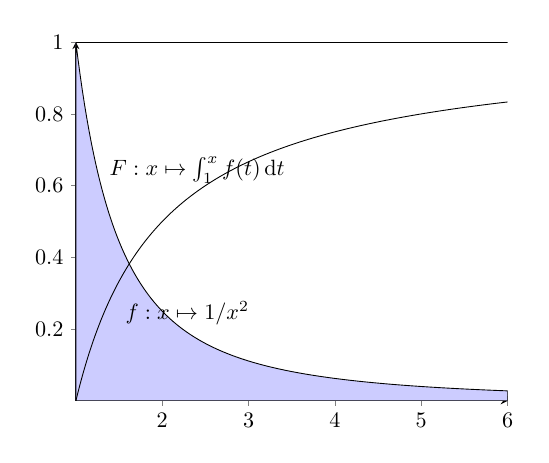
\begin{tikzpicture}[scale=0.8]
\begin{axis}[
	   axis y line = middle,
       axis x line = middle,
       samples     = 200,
       domain      = 0:1,
       xmin = 1, xmax = 6,
       ymin = 0, ymax = 1,
]
\addplot[domain=1:6,fill=blue!20] {1/(x^2)} node[pos=0.3,above] {$f: x\mapsto 1/x^2$}\closedcycle ;
\addplot[domain=1:6] {1-1/x} node[pos=0.3,above] {$F: x\mapsto \int_1^x f(t)\, \mathrm dt$};
\addplot[domain=1:6] {1} node[pos=0.3,above] {$M$};
\end{axis}
\end{tikzpicture}\\
$\int_a^b f(x)\,\mathrm dx$ converge car $F$ est majorée par 1.
\end{center}

\begin{center}
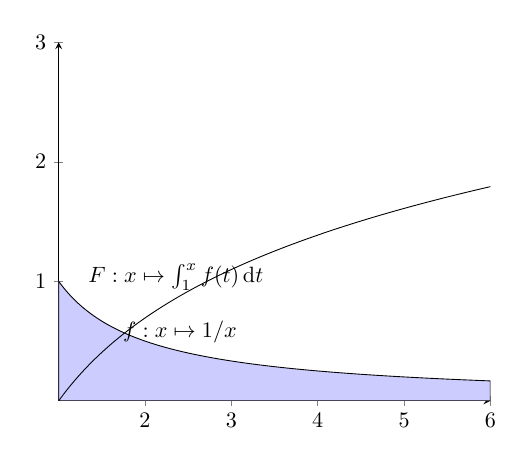
\begin{tikzpicture}[scale=0.8]
\begin{axis}[
	   axis y line = middle,
       axis x line = middle,
       samples     = 200,
       domain      = 0:1,
       xmin = 1, xmax = 6,
       ymin = 0, ymax = 3,
]
\addplot[domain=1:6,fill=blue!20] {1/(x)} node[pos=0.3,above] {$f: x\mapsto 1/x$}\closedcycle ;
\addplot[domain=1:6] {ln(x)} node[pos=0.3,above] {$F: x\mapsto \int_1^x f(t)\, \mathrm dt$};
\end{axis}
\end{tikzpicture}\\
$\int_a^b f(x)\,\mathrm dx$ diverge vers $+\infty$ car $F$ n'est pas majorée.
\end{center}
\end{Proposition}
\begin{Demonstration}
$F$ est croissante car $F'(x)=f(x)\geq 0$. D'après le théorème de
la limite monotone, $F$ admet une limite en $\infty$ qui est finie si et seulement si $F$ est majorée.
\end{Demonstration}
\subsection{Règles de convergence}
\begin{Theoreme}[Règle de comparaison]
Soit $f,g:[a,b[\to\R$ deux fonctions continues et positives tel que
$$\forall x\in [a,b[: f(x)\leq g(x).$$ 
Alors 
\begin{itemize}
\item
  si l'intégrale $\int_a^b g(x)\,\mathrm dx$ converge, alors l'intégrale $\int_a^b f(x)\,\mathrm dx$ converge également, et alors 
  $$  \int_a^b f(x)\,\mathrm dx \leq \int_a^b g(x)\,\mathrm dx,$$
\item
  si l'intégrale $\int_a^b f(x)\,\mathrm dx$ diverge, alors l'intégrale $\int_a^b g(x)\,\mathrm dx$ diverge également.
\end{itemize}
\end{Theoreme}
\begin{Demonstration}
Soit $t\in[a,b[$.
$$ \int_a^t f(x)\,\mathrm dx\overbrace{\leq}^{\text{coissance sur un segment}}\int_a^t g(x)\,\mathrm dx\overbrace{\leq}^{\text{Majoration du théorème de la limite monotome}}\int_a^b g(x)\,\mathrm dx.$$
Donc la fonction $F:t\mapsto \int_a^t f(x)\,\mathrm dx$ est croissante et majorée donc admet une limite en l'infini. Par passage à la limite, on  obtient : 
 $$  \int_a^b f(x)\,\mathrm dx \leq \int_a^b g(x)\,\mathrm dx.$$
\end{Demonstration}
\begin{Exemple}
Quelle est la nature de $\int_1^{+\infty}\frac{\sin^2(x)}{x^2+\sqrt{x}}  \,\mathrm dx$ ?\\
$x\mapsto \frac{\sin^2(x)}{x^2+\sqrt{x}}$ est continue et positive  sur $[1,+\infty[$. 
On a  
$$\forall t\in [1,+\infty[ :\quad  \frac{\sin^2(x)}{x^2+\sqrt{x}}\leq \frac{1}{x^2}.$$
Comme l'intégrale de Riemann $\int_1^{+\infty}\frac{1}{x^2 }\,\mathrm dx$ converge, $\int_1^{+\infty}\frac{\sin^2(x)}{x^2+\sqrt{x}}  \,\mathrm dx$ converge.\\
\end{Exemple}
\begin{Theoreme}[Règle de petit 0 et grand O]
Soit $f,g:[a,b[\to\R$ deux fonctions continues et positives tel que
$$ f(x)=\underset{ \overset { x \rightarrow b } {} } {o}(g(x))\text{ ou  }f(x)=\underset{ \overset { x \rightarrow b } {} } {O}(g(x))$$ 
Alors 
\begin{itemize}
\item
  si l'intégrale $\int_a^b g(x)\,\mathrm dx$ converge, alors l'intégrale $\int_a^b f(x)\,\mathrm dx$ converge également,
\item
  si l'intégrale $\int_a^b f(x)\,\mathrm dx$ diverge, alors l'intégrale $\int_a^b g(x)\,\mathrm dx$ diverge également.
\end{itemize}
\end{Theoreme}
\begin{Demonstration}
 Comme $ f(x)=\underset{ \overset { x \rightarrow b } {} } {o}(g(x))$, il existe $t\in[a,b[$ tel que $f(x)\leq g(x), \forall x\geq t.$ Comme $\int_t^b g(x)\,\mathrm dx$ converge, $\int_t^b f(x)\,\mathrm dx$ converge par règle de comparaison. $\int_a^b f(x)\,\mathrm dx$ converge par raccordement.
\end{Demonstration}
\begin{Exemple}
Quelle est la nature de $\int_1^{+\infty}\frac{\ln(x)}{x^2}  \,\mathrm dx$ ?\\
$x\mapsto \frac{\ln(x)}{x^2}$ est continue et positive  sur $[1,+\infty[$.
On a  
$$\frac{\ln(x)}{x^2} =\underset{ \overset { x \rightarrow +\infty} {} } {o}\left(\frac{1}{x^{3/2}}\right) $$
Comme l'intégrale de Riemann $\int_1^{+\infty}\frac{1}{x^{3/2}}\,\mathrm dx$ converge, $\int_1^{+\infty}\frac{\ln(x)}{x^2} \,\mathrm dx$ converge par règle du petit o.
\end{Exemple}
\begin{Theoreme}[Règle de l'équivalent]
Soit $f,g:[a,b[\to\R$ deux fonctions continues et de signe constant au voisinage de $b$ tel que
$$ f(x)\underset{ \overset { x \rightarrow b } {} } {\sim}g(x).$$ 
Alors les intégrales $\int_a^b f(x)\,\mathrm dx$ et $\int_a^b g(x)\,\mathrm dx$ sont de même nature.
\end{Theoreme}
\begin{Demonstration}
Supposons $f$ positive au voisinage de $b$. Comme $ f(x)\underset{ \overset { x \rightarrow b } {} } {\sim}g(x)$, il existe alors $t \in [a,b [$ 
tel que tel que $$\forall x\in [t,b[: \quad  \frac{1}{2}f(x)\leq g(x)\leq \frac{3}{2}f(x).$$
On conclut par application de la règle de comparaison.\\
Dans le cas négatif, la preuve est identique pour $-f$ et $-g$.
\end{Demonstration}

\begin{Exemple}
Quelle est la nature de $\int_0^{1}\frac{\sin(\sqrt{x})}{x^2}  \,\mathrm dx$ ?\\
$x\mapsto \frac{\sin(\sqrt{x})}{x}$ est continue et positive  sur $]0,1]$. On a \\
$$ \frac{\sin(\sqrt{x})}{x^2} \underset{ \overset { x \rightarrow 0 } {} }{\sim}\frac{\sqrt{x}}{x^2}=\frac{1}{x^{3/2}}.$$
Comme l'intégrale de Riemann $\int_0^1 \frac{1}{x^{3/2}}\,\mathrm dx$ diverge, $\int_0^{1}\frac{\sin(\sqrt{x})}{x^2}  \,\mathrm dx$ diverge par règle d'équivalent.
\end{Exemple}


\subsection{Comparaison série-intégrale}
Les séries sont un procédé de sommation de grandeurs discrètes, l'intégrale de grandeurs continues. L'analogie formelle entre les deux domaines permet de faire passer des idées intéressantes de l'une à l'autre. On compare ces deux objets mathématiques à l'aide d'inégalités.\\
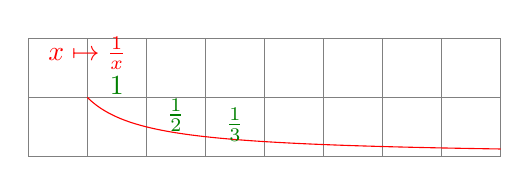
\begin{tikzpicture}[scale=0.75]
\tkzInit[xmax=8,ymax=2]
\tkzAxeXY
\tkzGrid
\draw (1,1.3) node[above,color=red]{$x\mapsto\frac 1 x $} ; 
\draw [domain=1:8,samples=200,color=red] plot (\x,{1/\x}); 
\tkzFct[color = black]{1./(x)}
\tkzDrawRiemannSumSup[fill=green!60,
                     opacity=.2,
                     color=green,
                     line width=1pt,
                     interval=1:8,
                     number=7] 
\foreach \x/\t in {1.5/$1$,2.5/$\frac12$,3.5/$\frac13$}
\node[green!50!black] at (\x,{(1/(\x-0.5))+0.2}){\t}; 
\end{tikzpicture}
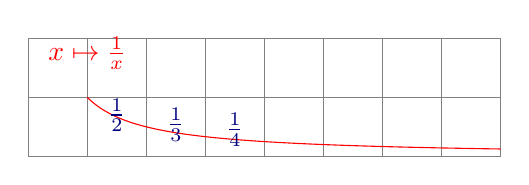
\begin{tikzpicture}[scale=0.75]
\tkzInit[xmax=8,ymax=2]
\tkzAxeXY
\tkzGrid
\draw (1,1.3) node[above,color=red]{$x\mapsto \frac 1 x $} ; 
\draw [domain=1:8,samples=200,color=red] plot (\x,{1/\x});  
\tkzFct[color = black]{1./(x)}
\tkzDrawRiemannSumInf[fill=blue!60,
                     opacity=.2,
                     color=blue,
                     line width=1pt,
                     interval=1:8,
                     number=7] 
\foreach \x/\t in {1.5/$\frac12$,2.5/$\frac13$,3.5/$\frac14$}
\node[blue!50!black] at (\x,{(1/(\x+0.5))+0.2}){\t}; 
\end{tikzpicture} \\
L'aire entre $1$ et $n$ est:
\begin{itemize}
\item sous la courbe rouge   : $\int_1^N f(x)dx$,
\item des rectangles verte  : $\sum_{n=1}^{N-1}f(n)$,
\item  des rectangles bleues  : $\sum_{n=2}^{N}f(n)$.
\end{itemize}
Géométriquement, on a les inégalités :
$$\sum_{n=2}^{N}f(n) \leq \int_1^N f(x)\,\mathrm dx \leq \sum_{n=1}^{N-1}f(n).$$
Si $\sum f(n)$ diverge alors $t\mapsto \int_1^t f(x)\,\mathrm dx$ n'est pas majorée. Comme $t\mapsto \int_1^t f(x)\,\mathrm dx$ est croissante,  $\int_a^{+\infty} f(x)\,\mathrm dx$ converge. Idem si $\sum f(n)$ diverge.\\
En conclusion, la série $\sum f(n)$ converge si et seulement si l'intégrale  $\int_a^{+\infty} f(x)\,\mathrm dx$ converge.
\begin{Theoreme}[Comparaison séries/intégrales]
Soit $f$ une application continue, positive et décroissante sur $[a,+\infty[$.\\
Alors la série $\sum_{n\geq a} f(n)$ et l'intégrale $\int_a^{+\infty} f(x)\,\mathrm dx$ sont de même nature.
\end{Theoreme}

Une application directe de ce théorème nous donne de nouvelles séries de référence.
\begin{Theoreme}[Séries de Riemann]
Soit $\alpha \in \R$.\\
$\sum_n \frac{1}{n^\alpha}$ converge si et seulement si $\alpha > 1$.
\end{Theoreme}
\begin{Demonstration}
On a :\\
\begin{itemize}
\item $\alpha\leq 0$ : comme  $\lim\limits_{n\to\infty} \frac{1}{n^\alpha}\neq 0$, la série diverge grossièrement.
\item $\alpha>0$ : la fonction $x\mapsto \frac{1}{x^\alpha}$ est continue, positive et décroissante sur $[1,+\infty[$, l'intégrale  $\int_1^{+\infty}\frac{1}{x^\alpha}  \,\mathrm dx$
et la série $\sum_n \frac{1}{n^\alpha}$ sont de même nature. Donc la série converge si et seulement si   $\alpha > 1$.
\end{itemize}
\end{Demonstration}
\section{Intégrale de fonctions réelles de signe variable}
\subsection{Absolument convergente}
Nous passons maintenant à l'étude d'intégrale de fonctions réelles de signe variable. Pour expliquer le titre de cette section,
 il convient de remarquer que si le signe de $f$ est constant
à partir d'un certaine valeur $c$, l'étude de la convergence de $\int_a^b f(x)\,\mathrm dx$ se ramène à celle d'une
intégrale de signe constant. En effet,  $\int_a^b f(x)\,\mathrm dx$ et $\int_c^b f(x)\,\mathrm dx$ sont de même nature.\\
Ce que nous allons voir dans cette section n'est donc réellement nouveau que pour les intégrales de fonctions qui changent de signe
une infinité de fois.\\
Une première idée pour l'étude des intégrales de signe variable est de décomposer la fonction $f$ sur sa partie positive et négative $f = f^+-f^-$ où $$\forall x\in [a,b[:\quad f^+(x)=\max(f(x),0)\text{ et } f^-(x)=\max(-f(x),0).$$
\begin{center}
\begin{tikzpicture}[scale=0.5]
\begin{axis}[
	   axis y line = middle,
       axis x line = middle,
       samples     = 200,
       domain      = 0:1,
       xmin = 0, xmax = 1.5,
       ymin = -1, ymax = 1,
]
\addplot[domain=0:1.5] {1-(x^2)} node[pos=0.3,above] {$f$} ;
\end{axis}
\end{tikzpicture}
\begin{tikzpicture}[scale=0.5]
\begin{axis}[
	   axis y line = middle,
       axis x line = middle,
       samples     = 200,
       domain      = 0:1,
       xmin = 0, xmax = 1.5,
       ymin = -1, ymax = 1,
]
\addplot[domain=0:1,color = red] {1-(x^2)} node[pos=0.3,above] {$f^+$} ;
\addplot[domain=1:1.5,color = red] {0)}  ;
\end{axis}
\end{tikzpicture}
\begin{tikzpicture}[scale=0.5]
\begin{axis}[
	   axis y line = middle,
       axis x line = middle,
       samples     = 200,
       domain      = 0:1,
       xmin = 0, xmax = 1.5,
       ymin = -1, ymax = 1,
]
\addplot[domain=1:1.5,color = blue] {-1+(x^2)} node[pos=0.3,above] {$f^-$} ;
\addplot[domain=0:1,color = blue] {0)}  ;
\end{axis}
\end{tikzpicture}
\end{center}
Soit $c\in [a,b[$. L'intégrale sur le segment $[a,c]$ est :
$$ \int_a^v f(x)\,\mathrm dx= \int_a^c (f^+(x)-f^-(x))\,\mathrm dx = \int_a^c f^+(x)\,\mathrm dx -  \int_a^c f^-(x))\,\mathrm dx.$$
Par passage à la limite, une condition suffisante pour que $\int_a^v f(x)\,\mathrm dx$ converge  et que les deux intégrales $\int_a^b f^+(x)\,\mathrm dx$  et $\int_a^b f^-(x)\,\mathrm dx$ convergent. \\
Compte tenu des inégalités $$0\leq f^+ \leq |f| , \quad 0\leq f^- \leq |f|,$$ le
théorème de comparaison des intégrales à fonctions positives nous permet de conclure qu'une
condition suffisante pour la convergence de $\int_a^b f^+(x)\,\mathrm dx$ et $\int_a^b f^-(x)\,\mathrm dx$
et donc aussi $\int_a^b |f(x)|\,\mathrm dx$ converge. Nous venons ainsi d'établir le résultat le plus important pour
la convergence d'une intégrale de fonctions réelles de signe variable.
\begin{Theoreme}
Si $\int_a^b |f(x)|\,\mathrm dx$ converge alors $\int_a^b f(x)\,\mathrm dx$ converge.
\end{Theoreme}
\begin{Definition}[Absolue convergence]
Soit $f : [a,b [\to \R$ continue sur $[a,b[$.\\
On dit que $\int_a^b f(x)\,\mathrm dx$ est \defi{absolument convergente} lorsque 
$\int_a^b |f(x)|\,\mathrm dx$ converge.
\end{Definition}
\begin{Exemple} Démontrons que  $\int_1^{+\infty } \frac{\sin x}{x^2}\,\mathrm dx$ est absolument convergente. On a :
$$\forall x \in [1,{+\infty }[ : \left| \frac{\sin x}{x^2}\right|\leq \frac{1}{x^2}.$$ 
Comme  $\int_1^{+\infty}\frac{1}{x^2 }\,\mathrm dx$ est convergente par intégrale de Riemann, l'intégrale $\int_1^{+\infty } \frac{\sin x}{x^2}\,\mathrm dx$ est absolument convergente.
\end{Exemple}
\begin{Theoreme}
Une intégrale absolument convergente est convergente.
\end{Theoreme}
\begin{Definition}[Intégrable]
Soit $f : I\to \R$ continue sur $I$.\\
On dit que $f$ est \defi{intégrable} sur $I$ si 
$\int_I f(x)\,\mathrm dx$ est absolument convergente.
\end{Definition}
\begin{Proposition}[Espace vectoriel]
L'ensemble des fonctions continues et intégrables sur $I$ est un espace vectoriel.
\end{Proposition}
\begin{Definition}[Semi-convergente]
Une intégrale convergente mais non absolument convergente est dite \defi{semi-convergente}.
\end{Definition}
\begin{Exemple}[Intégrale de Dirichlet]
L'intégrale $\int_0^{+\infty } \frac{\sin x}{x}\,\mathrm dx$ est semi-convergente.
\begin{itemize}
\item Non absolument convergente :\\
$f : x \mapsto \frac{\sin x}{x}$ est continue sur $\mathbb R^+$ en la prolongeant par continuité en $0$ en posant $f (0) = 1$.\\
On a :
$$\forall n \in  \N:\quad \int_{n\pi}^{(n+1)\pi}\left|\frac{\sin x}{x}\right|\,\mathrm dx \geq \inf_{x\in [n\pi,(n+1)\pi] }\frac{1}{|x|}\times  \int_{n\pi}^{(n+1)\pi} |\sin x|  \,\mathrm dx  =\frac{1}{(n+1)\pi}\times 2.$$
D'où : 
$$\forall p \in   \N :\quad \int_{0}^{p\pi}\left|\frac{\sin x}{x}\right|\,\mathrm dx  \geq \sum_{n=0}^{p-1}\frac{2}{(n+1)\pi}\overbrace{\xrightarrow[p\to\infty]{}}^{\text{Série harmonique}}+\infty . $$
\item Convergente :\\
Par intégration par parties,  les fonctions $u : x \mapsto 1 - \cos x$ et $v : x \mapsto 1/x$ sont $C^1$ sur $\mathbb R^{+*}$ et le produit $u.v$ admet des limites finies en 0 et en $+\infty$, donc les intégrales $\int_{0}^{+\infty}u'(x)v(x)\,\mathrm dx$ et $\int_{0}^{+\infty}u(x)v'(x)\,\mathrm dx$ sont de même nature.\\
Or $\int_0^{+\infty } \frac{\cos x-1}{x^2}\,\mathrm dx$ est absolument convergente sur $\mathbb R^{+*}$ par règle de comparaison. Donc l'intégrale  $\int_0^{+\infty } \frac{\sin x}{x} \,\mathrm dx$ converge également. 
\end{itemize}
\end{Exemple}
\begin{Proposition}[Inégalité de la moyenne]
Soit $f : [a,b [\to \R$ continue sur $\K$ telle que $\int_a^b f(x)\,\mathrm dx$ est absolument convergente.
\\
Alors 
$$\left| \int_a^b f(x)\,\mathrm dx \right| \leq  \int_a^b \left| f(x) \right| \,\mathrm dx.$$
\end{Proposition}
\begin{Demonstration}
Comme $\int_a^b f(x)\,\mathrm dx$ est absolument convergente,  $\int_a^b f(x)\,\mathrm dx$ et  $\int_a^b -f(x)\,\mathrm dx$ sont convergentes. On a :
$$\forall x \in [a,b[:\quad f(x)\leq |f(x)| \text{ et } -f(x)\leq |f(x)| $$
On obtient l'inégalité car  $ \int_a^b f(x)\,\mathrm dx \leq  \int_a^b \left| f(x) \right| \,\mathrm dx.$ et $- \int_a^b f(x)\,\mathrm dx \leq  \int_a^b \left| f(x) \right| \,\mathrm dx.$.
\end{Demonstration}

%
%
%
%\subsection{Espace préhilbertien}
%
%\Para{Définition} Soit $\Fn fI\K $ et $\Fn gI\K $ continues. On dit que $f$ est  de carré intégrable si $\int_I |f|^2$ est convergente. Dans ce cas, on note  $\int_I |f|^2<+\infty$. L'ensemble des fonctions continues de carré intégrables sur $I$ est noté $\mathcal{L}^2(I)$.
%
%\Para{Exemple} La fonction $f$ définies sur $\mathbb{R}^{+*}$ par $f:t\mapsto \frac{1}{1+t}$ est continue et de carré intégrable sur $\mathbb{R}^{+*}$. Cependant elle est non intégrables sur $\mathbb{R}^{+*}$.\\
% La fonction $g$ définies sur $]0,1]$ par $g:t\mapsto \frac{1}{\sqrt{t}}$ est continue et intégrables sur $]0,1]$. Cependant, elle n'est pas de carré intégrable $]0,1]$. Cependant elle est non 
%
%\Para{Proposition} $\mathcal{L}^2(I)$ est un espace vectoriel.
%
%\Para{Lemme} Soit $f, g \in \mathcal{L}^2(I) $.\\
%Alors $fg$ est intégrable.
%
%
%\Para{Définition}[Produit scalaire] L'application $$\Fonction{\langle .,. \rangle }{\mathcal{L}^2(I)\times \mathcal{L}^2(I) }{\mathbb{R}}{f,g}{\int_I fg}$$
%est un produit scalaire sur l'espace vectoriel des fonctions continues de carré intégrable. 
%
%\Para{Définition}[Norme]La norme définie par ce produit scalaire est appelée \emph{norme de la convergence en moyenne quadratique} et noté $N_2$,
%$$\forall f \in \mathcal{L}^2(I), N_2(f)=\sqrt{\PS{f}{f}}= \sqrt{\int_I f^2}.$$
%
%\Para{Proposition}[Inégalité de Cauchy-Schwartz] Soit $f, g \in \mathcal{L}^2(I) $.\\
%Alors $$\left|\PS f g \right| \leq N_2(f)N_2(g)$$ $$|\int_I fg |\leq \sqrt{\int_I f^2}\sqrt{\int_I g^2}.$$
%
%
%

%

%
%
%
%\section{Annexe}
%
%\subsection{Intégration sur un segment}
%
%\subsubsection{Subdivisions}
%
%\Para{Définition}
%
%Soit $\IntF{a,b}?\R $ un segment.
%Une \emph{subdivision} de $[a,b]$ est un $(n+1)$-uplet
%$\nUplet\sigma 0n\in \R ^{n+1}$ tel que
%\[a =\sigma _0 <\sigma _1 < \cdots <\sigma _n = b\]
%
%\Para{Définitions}
%
%Soit $f \colon \IntF{a,b} \to E$.
%\begin{itemize}
%\item $f$ est dite \emph{en escaliers} sur $\IntF{a,b}$
%  si et seulement si il existe une subdivision $\nUplet\sigma 0n$ de $\IntF{a,b}$ telle que
%  pour tout $k\in \Dcro{0,n-1}$,
%  $f$ est constante sur $\intO{\sigma _k,\sigma _{k+1}}$.
%\item $f$ est dite \emph{continue par morceaux} sur $\IntF{a,b}$
%  si et seulement si il existe une subdivision $\nUplet\sigma 0n$ de $\IntF{a,b}$ telle que
%  pour tout $k\in \Dcro{0,n-1}$,
%  la restriction de $f$ à $\intO{\sigma _k,\sigma _{k+1}}$ est continue
%  \emph{et se prolonge en une fonction continue sur $\intF{\sigma _k,\sigma _{k+1}}$}.
%\item Plus généralement,
%  $f$ est dire \emph{de classe $\CC k$ par morceaux} sur $\IntF{a,b}$
%  si et seulement si il existe une subdivision $\nUplet\sigma 0n$ de $\IntF{a,b}$ telle que
%  pour tout $k\in \Dcro{0,n-1}$,
%  la restriction de $f$ à $\intO{\sigma _k,\sigma _{k+1}}$ est de classe $\CC k$
%  \emph{et se prolonge en une fonction de classe $\CC k$ sur $\intF{\sigma _k,\sigma _{k+1}}$}.
%\end{itemize}
%
%\Para{Théorème}
%
%Soit $f \colon [a,b] \to E$ continue par morceaux et $?> 0$.
%Alors il existe $?\colon [a,b] \to E$ en escaliers
%tel que $\forall x\in [a,b]\+ \Norm{f(x) -?(x)}\leq  ?$.
%
%\subsubsection{Intégration sur un segment (rappel première année)}
%
%\Para{Remarque}
%
%La construction de l'intégrale n'est pas fondamentale,
%je renvoie donc au cours de première année.
%On pourra toutefois noter que les propriétés suivantes
%\emph{caractérisent} l'intégrale des fonctions continues par morceaux
%sur un segment:
%\begin{itemize}
%\item Intégrale d'une fonction constante,
%\item Relation de Chasles,
%\item Inégalité de la moyenne,
%\item Croissance.
%\end{itemize}
%
%\subsubsection{Propriétés de l'intégrale}
%
%\Para{Proposition}[intégrale d'une fonction constante]
%
%Soit $f \colon I \to E$ une fonction, $(a,b)\in I^2$ où $a\leq  b$.
%On suppose que
%\[\exists C\in E\+\forall x\in \IntO{a,b}\+ f(x) = C.\]
%Alors $f$ est continue par morceaux sur $\IntF{a,b}$ et \[\int_a^b f = (b-a)C.\]
%
%\Para{Proposition}[linéarité]
%
%Soit $f, g \colon I \to E$ deux fonctions continues par morceaux, $(a,b)\in I^2$ et $(\lambda ,\mu )\in \K ^2$.
%Alors $\lambda f +\mu g \colon I \to E$ est continue par morceaux sur $I$ et
%\[\int_a^b (\lambda f +\mu g) =\lambda \int_a^b f +\mu \int_a^b g.\]
%
%\Para{Proposition}[relation de Chasles]
%
%Soit $f \colon I \to E$ une fonction continue par morceaux et $(a,b,c)\in I^3$.
%Alors \[\int_a^b f =\int_a^c f +\int_c^b f.\]
%
%\Para{Proposition}[inégalité de la moyenne]
%
%Soit $f \colon I \to E$ une fonction continue par morceaux,
%$(a,b)\in I^2$ où $a\leq  b$.
%Alors \[\left\| \int_a^b f(t) \D t \right\| \leq  \int_a^b \Norm{f(t)} \D t.\]
%
%\Para{Remarque}
%
%Si l'on enlève l'hypothèse $a\leq  b$, la conclusion s'écrit alors
%\[\left\| \int_a^b f(t) \D t \right\| \leq  \left| \int_a^b \Norm{f(t)} \D t \right|.\]
%
%\Para{Proposition}[positivité]
%
%Soit $f \colon I \to \Rp$ une fonction continue par morceaux,
%$(a,b)\in I^2$ où $a\leq  b$.
%Alors \[\int_a^b f\geq  0.\]
%
%\Para{Proposition}[croissance]
%
%Soit $f, g \colon I \to\R $ deux fonctions continues par morceaux,
%$(a,b)\in I^2$ où $a\leq  b$.
%On suppose que
%\[\forall x\in [a,b]\+ f(x)\leq  g(x).\]
%Alors
%\[\int_a^b f\leq  \int_a^b g.\]
%
%\Para{Théorème}[stricte positivité]
%
%Soit $f \colon I \to \Rp$ une fonction \emph{continue},
%$(a,b)\in I^2$ où $a\leq  b$.
%On suppose que
%\[\int_a^b f = 0.\]
%Alors $f$ est identiquement nulle sur $\IntF{a,b}$.
%
%\Para{Théorème}[inégalité de Cauchy-Schwarz]
%
%Soit $f, g \colon I \to\K $ deux fonctions continues par morceaux
%et $(a,b)\in I^2$.
%Alors
%\[\left|\int_a^b f(t) g(t) \D t \right|\leq  
%  ?{\int_a^b \Abs{f(t)}^2 \D t}
%?{\int_a^b \Abs{g(t)}^2 \D t}.\]
%Si l'on suppose en outre que $f$ et $g$ sont continues,
%alors il y a égalité si et seulement si la famille $(f,g)$ est liée.
%
%\Para{Définition}
%
%Soit $f \colon [a,b] \to E$ continue par morceaux.
%La \emph{valeur moyenne} de $f$ sur $[a,b]$ est $\frac{1}{b-a}\int_a^b f$.
%
%\subsubsection{Sommes de Riemann}
%
%\Para{Théorème}
%
%Soit $f \colon [a,b] \to E$ continue par morceaux.
%Soit $(\sigma _n)_{n\in \N }$ une suite de subdivisions de $[a,b]$.
%On note $\sigma _n$ la subdivision
%\[a = ?_{n,1} < ?_{n,2} < \dots < ?_{n,m_n} = b.\]
%On note $h_n$ le pas de la subdivision $\sigma _n$, c.-à-d.
%\[h_n = \max_{1\leq  k<m_n} \Bigl( ?_{n,k+1} - ?_{n,k} \Bigr).\]
%On suppose que $h_n \to 0$.
%Alors
%\[\frac{1}{m_n} \sum_{k=1}^{m_n} f(?_{n,k}) \Toninf \int_a^b f(t) \D t.\]
%
%\Para{Corollaire}
%
%Soit $f \colon [0,1] \to E$ continue par morceaux.
%Alors
%\[\frac{1}{n+1} \sum_{k=0}^{n} f\left(\frac{k}{n}\right) \Toninf \int_0^1 f.\]
%
%\subsubsection{Primitives}
%
%\Para{Définition}
%
%Soit $f \colon I \to E$. Une \emph{primitive} $F$ de $f$ sur $I$
%est une fonction dérivable sur $I$ telle que $F' = f$.
%
%\Para{Proposition}
%
%Soit $f \colon I \to E$ une fonction admettant deux primitives $F$ et $G$.
%Alors \[\exists C\in E\+\forall x\in I\+ F(x) - G(x) = C.\]
%
%Autrement dit, \emph{sur un intervalle}, deux primitives d'une
%même fonctions diffèrent d'une constante.
%
%\Para{Théorème}
%
%Soit $f \colon I \to E$ une fonction continue par morceaux et $a\in I$.
%On pose \[\Fonction{?}{I}{E}{x}{\int_a^x f(t) \D t.}\]
%Alors $?$ est continue sur $I$.
%De plus, si $f$ est continue en $x\in I$, alors
%$?$ est dérivable en $x$ et $?'(x) = f(x)$.
%
%\Para{Corollaire}
%
%Toute fonction continue sur un intervalle admet des primitives sur
%cet intervalle.
%
%\subsection{Fonctions continues par morceaux}
%
%\Para{Définition}
%
%Une \emph{subdivision} de $[a,b]$ est un $(n+1)$-uplet $\nUplet\sigma 0n\in \R ^{n+1}$ tel que:
%\[ a = \sigma _0 < \sigma _1 < \sigma _2 < \cdots < \sigma _{n-1} < \sigma _n = b. \]
%
%\Para{Définition}
%
%Soit $\Fn{f}{[a,b]}{\K }$.
%
%On dit que $f$ est \emph{continue par morceaux} sur le segment $[a,b]$
%£ssil. existe une subdivision $(\sigma _k)_{0\leq  k\leq  n}$ de $[a,b]$ telle que
%pour tout $k\in \Dcro{0,n-1}$, en notant $f_k$ la restriction de $f$ à l'intervalle ouvert $\intO{\sigma _k,\sigma _{k+1}}$, on ait:
%\begin{enumerate}
%\item
%  $f_k$ est continue sur l'intervalle ouvert $\intO{\sigma _k,\sigma _{k+1}}$,
%\item
%  $f_k$ se prolonge en une fonction continue, notée $\tilde f_k$ sur l'intervalle fermé $[\sigma _k,\sigma _{k+1}]$.
%\end{enumerate}
%
%\Para{Définition}
%
%Soit $I$ un intervalle quelconque de $\R $.
%On dit que $f$ est \emph{continue par morceaux sur $I$} si $f$ est continue par morceaux sur tout segment $K$ inclus dans $I$.
%On peut noter que cela correspond à la définition précédente si $I$ est un segment.
%
%\Para{Proposition}
%
%Soit $\Fn{f}{I}{\K }$ une fonction continue.
%Alors $f$ est continue par morceaux sur $I$.
%
%\Para{Proposition}
%
%L'ensemble $\mathcal{CM}(I,\K )$ des fonctions continues par morceaux de $I$ dans $\K $ est un sous-espace vectoriel de $\K ^I$.
%
%\Para{Proposition}
%
%Soit $\Fn{f}{I}{\K }$ une fonction continue par morceaux.
%Alors $f$ est bornée sur tout segment $K?I$.
%
%\Para{Définition}
%
%Soit $\Fn{f}{[a,b]}{\K }$ une fonction continue par morceaux.
%Soit $a =\sigma _0 <\sigma _1 < \dots <\sigma _n = b$ une subdivision adaptée.
%Pour $k\in \Dcro{0,n-1}$, on note $\tilde f_k$ l'unique fonction continue $[\sigma _k,\sigma _{k+1}] \to \K $ dont la restriction à l'ouvert $\intO{\sigma _k,\sigma _{k+1}}$ est égale à $f$.
%Par définition, l'intégrale de $f$ sur $[a,b]$ vaut
%\[ \int_a^b f =\sum_{k=0}^{n-1}\int_{\sigma _k}^{\sigma _{k+1}} \tilde f_k. \]
%
%On pose également $\int_b^a f = -\int_a^b f$.
%
%\Para{Proposition}[propriétés de l'intégrale]
%
%\begin{enumerate}
%\item
%  \emph{Linéarité}
%
%  Soit $f$ et $g$ deux fonctions continues par morceaux de $[a,b]$ dans $\K $.
%  Soit $(\lambda ,\mu )\in \K ^2$.
%  Alors $\int_a^b (\lambda f+\mu g) = \lambda \int_a^b f + \mu \int_a^b g$.
%\item
%  \emph{Relation de Chasles}
%
%  Soit $\Fn{f}{I}{\K }$ continue par morceaux et $(a,b,c)\in I^3$.
%  Alors $\int_a^c f = \int_a^b f + \int_b^c f$.
%\item
%  \emph{Positivité}
%
%  Soit $\Fn{f}{[a,b]}{\Rp}$ continue par morceaux.
%  Alors $\int_a^b f \geq  0$.
%\item
%  \emph{Stricte positivité}
%
%  Soit $\Fn{f}{[a,b]}{\Rp}$ une fonction \emph{continue}.
%  Si $\int_a^b f = 0$, alors $f = \tilde0$.
%\item
%  \emph{Croissance}
%
%  Soit $f, g \colon [a,b] \to \R $ continues par morceaux.
%  On suppose $\forall x\in \intO{a,b}$, $f(x)\leq  g(x)$.
%  Alors $\int_a^b f \leq  \int_a^b g$.
%\item
%  \emph{Inégalité de la moyenne}
%
%  Soit $\Fn{f}{[a,b]}{\K }$ continue par morceaux.
%  Alors $\left| \int_a^b f \right| \leq  \int_a^b \Abs{f}$.
%\end{enumerate}
%
%\Para{Remarque}
%
%La stricte positivité n'est pas valable pour les fonctions continues par morceaux. On a cependant ce résultat:
%
%\Para{Proposition}
%
%Soit $\Fn{f}{[a,b]}{\Rp}$ une fonction \emph{continue par morceaux}.
%Si $\int_a^b f = 0$, alors $\Ensemble{x\in [a,b]}{f(x)?0}$ est un ensemble fini.
\end{document}
